\section{Results}

\frame{
\frametitle{Status Quo}
1 file to test with: ``solarsystem.csv''
\begin{figure}
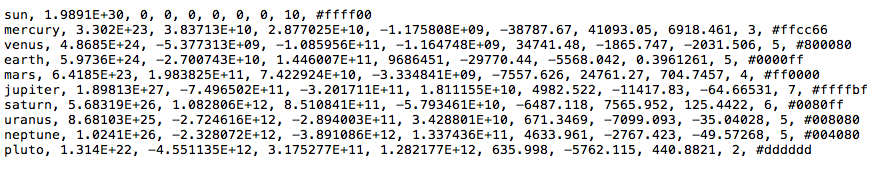
\includegraphics[scale=0.21]{solarsystem.png}
\end{figure}
\begin{figure}
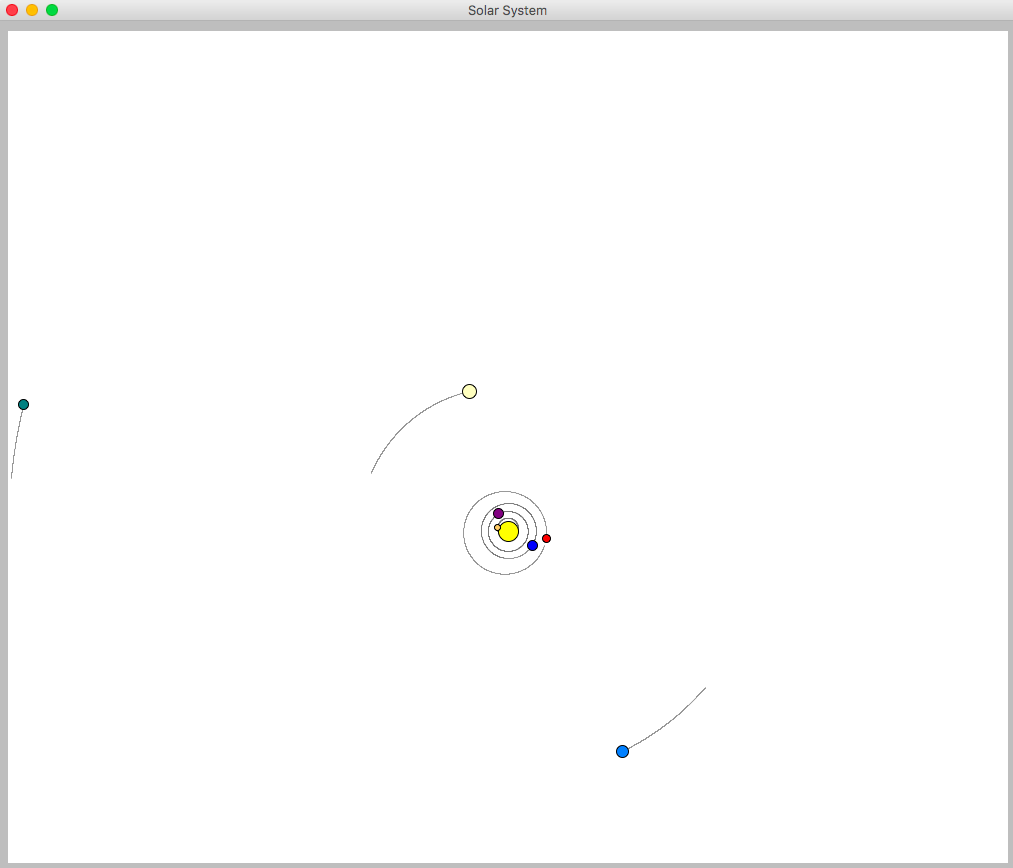
\includegraphics[scale=0.15]{original-orbits.png}
\end{figure}
}

\frame{
\frametitle{Multiple Test Cases}
\begin{figure}
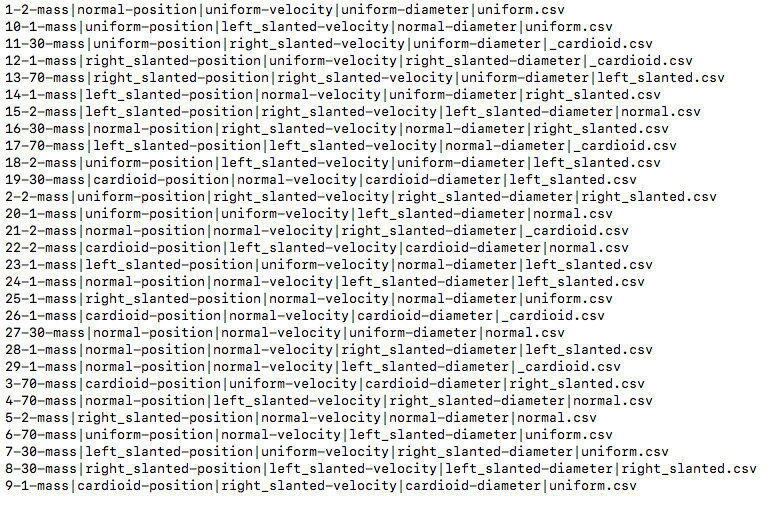
\includegraphics[scale=0.4]{many-files.png}
\end{figure}
}

\frame{
\frametitle{Orbits Simulation}
13-70-mass$|$right\_slanted-position$|$right\_slanted-velocity$|$uniform-diameter$|$left\_slanted.csv
\begin{itemize}
\item Case 13
\item 70 bodies
\item Mass - right-slant
\item Position - right-slant
\item Velocity - uniform
\item Diameter - left-slant
\end{itemize}
}

\frame{
\frametitle{Starting Orbits}
\begin{figure}
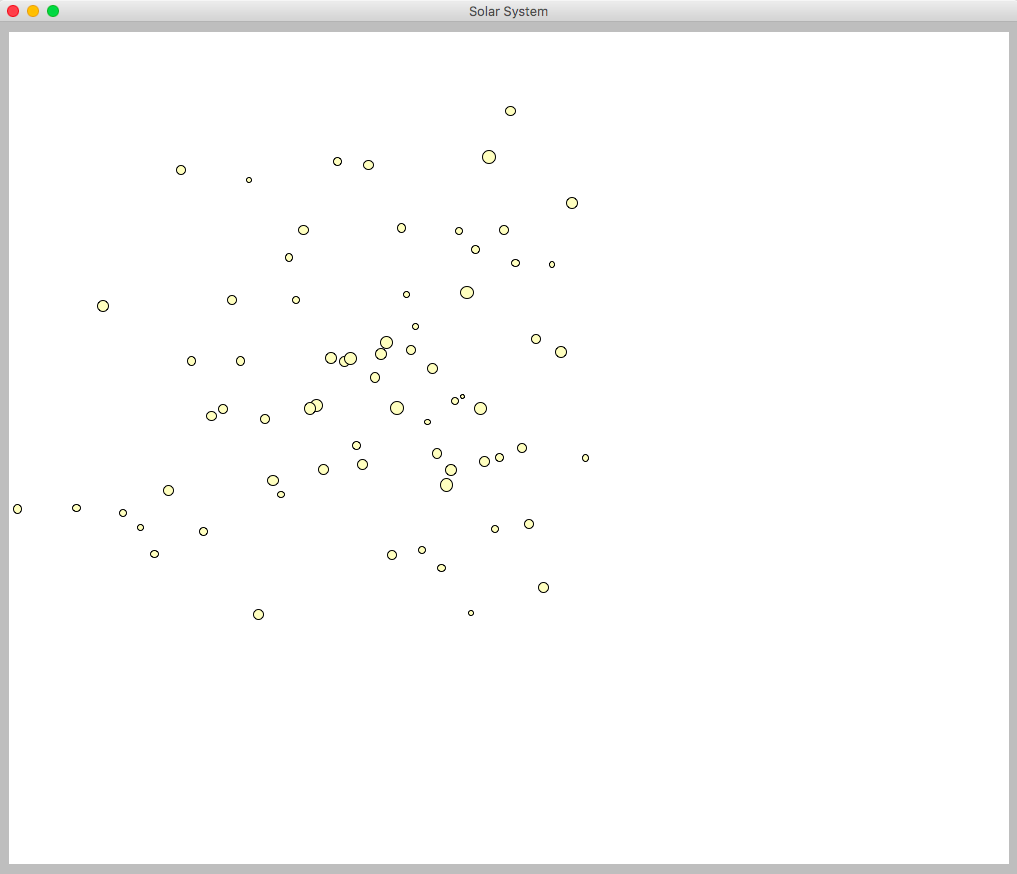
\includegraphics[scale=0.21]{start-ex.png}
\end{figure}
}

\frame{
\frametitle{Starting Observations}
\begin{itemize}
\item Sizes are mostly small-medium (from left-slant distribution)
\item Locations are clustered (from right-slant distribution)
\end{itemize}
}

\frame{
\frametitle{Ending Orbits}
665 time steps
\begin{figure}
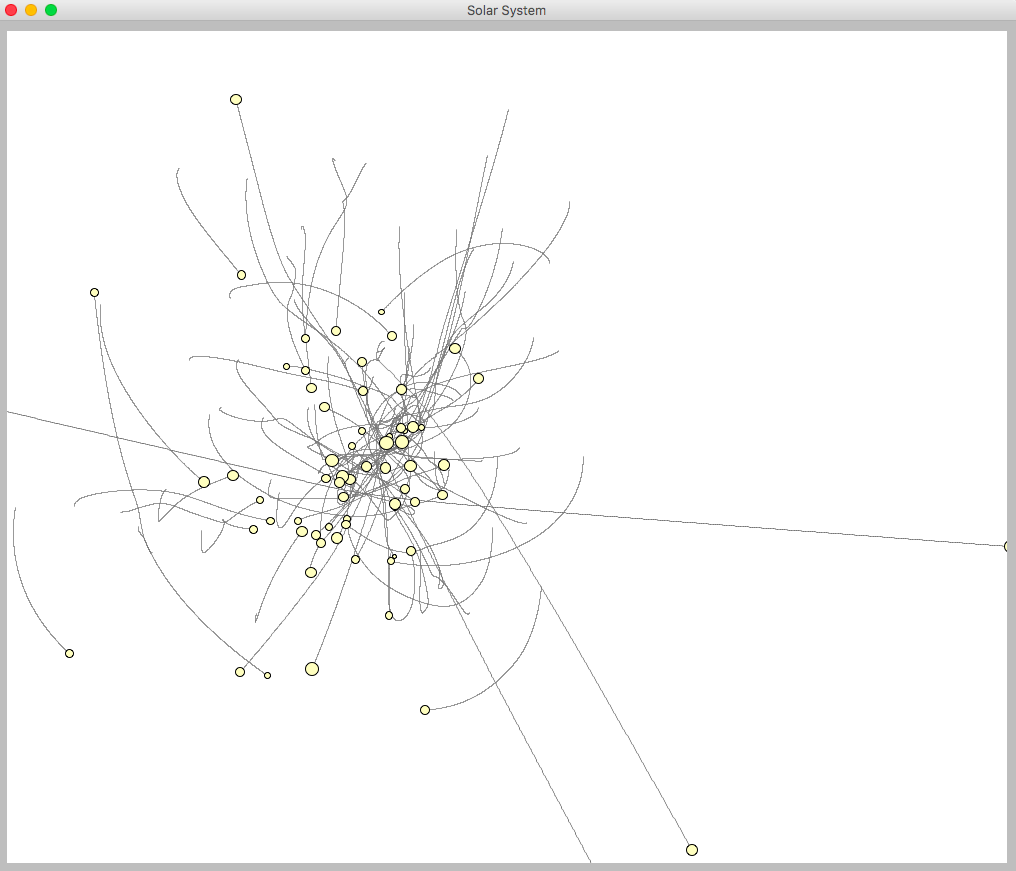
\includegraphics[scale=0.21]{final-ex.png}
\end{figure}
}

\frame{
\frametitle{Ending Observations}
\begin{itemize}
\item Behavior of gravity 
\item Path lengths are all different (from uniform velocity)
\end{itemize}
}



%%%%%%%%%%%%%%%%%%%%%%%%%%%%%%%%%%%%%%%%%%%%%%%%%%%%%%%%%%%%%%%%%%%%%%%%%%%%%%%%%%%%%%%%

\frame{
\frametitle{Earthquake Analysis}
6-70-magnitudes$|$cardioid-latitudes$|$left\_slanted-longitudes$|$right\_slanted-depths$|$cardioid.csv
\begin{itemize}
\item Case 6
\item 70 quake events
\item Magnitude \& Depth - Cardioid relationship
\item {Trend: High Magnitude $\to$ High Depth
\item Low Magnitude $\to$ Low Depth}
\item Latitudes - left-slant
\item Longitudes - right-slant
\end{itemize}
}

\frame{
\frametitle{\textbf{Magnitudes} \& Depths}
\begin{figure}
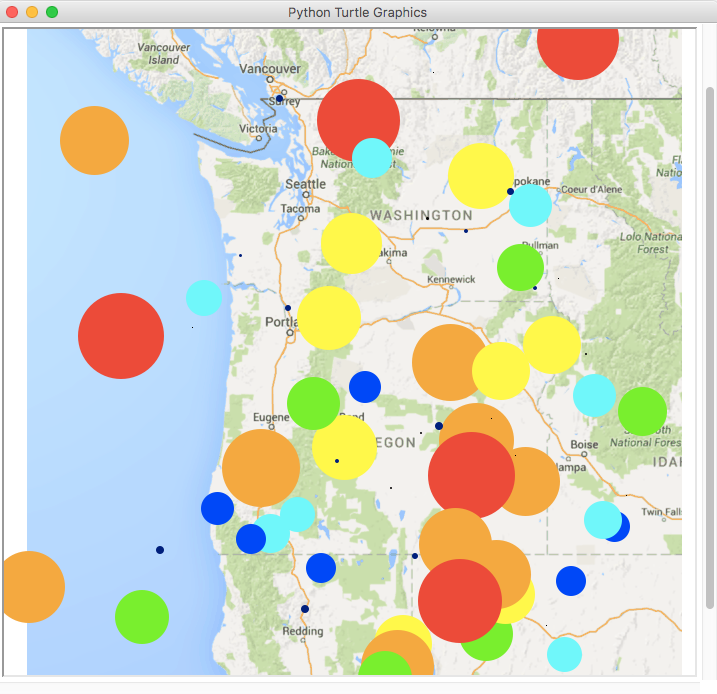
\includegraphics[scale=0.4]{mags.png}
\end{figure}
}

\frame{
\frametitle{Magnitudes \& \textbf{Depths}}
\begin{figure}
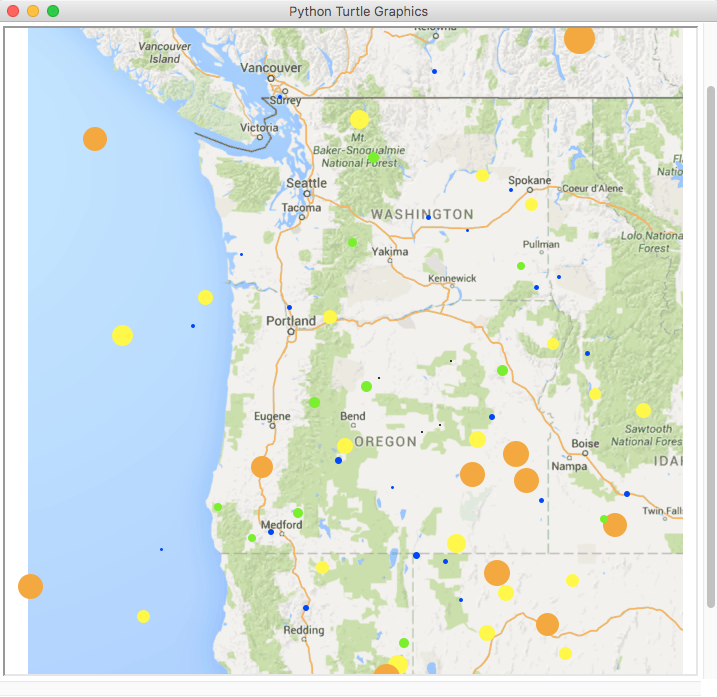
\includegraphics[scale=0.4]{depths.png}
\end{figure}
}

\frame{
\frametitle{Observations}
\begin{itemize}
\item Mostly predicted events?
\item Any outliers?
\end{itemize}
}


\frame{
\frametitle{\textbf{Magnitudes} \& Depths Frequent Occurrence}
\begin{figure}
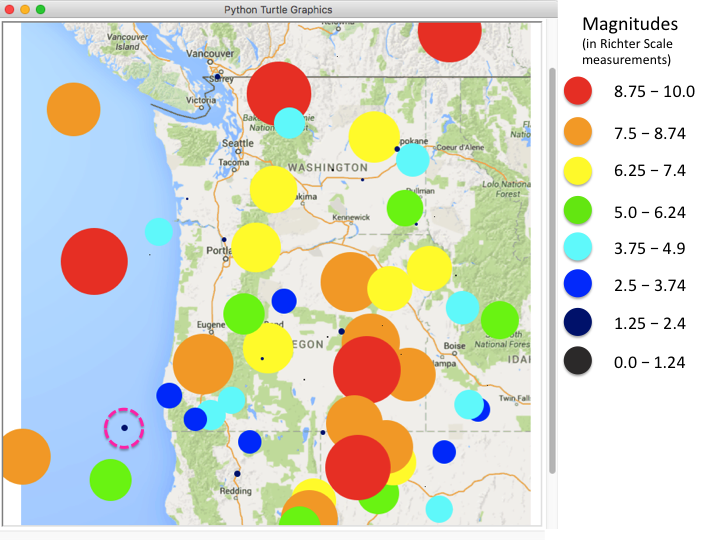
\includegraphics[scale=0.4]{mags-frequent-1.png}
\end{figure}
}

\frame{
\frametitle{Magnitudes \& \textbf{Depths} Frequent Occurence}
\begin{figure}
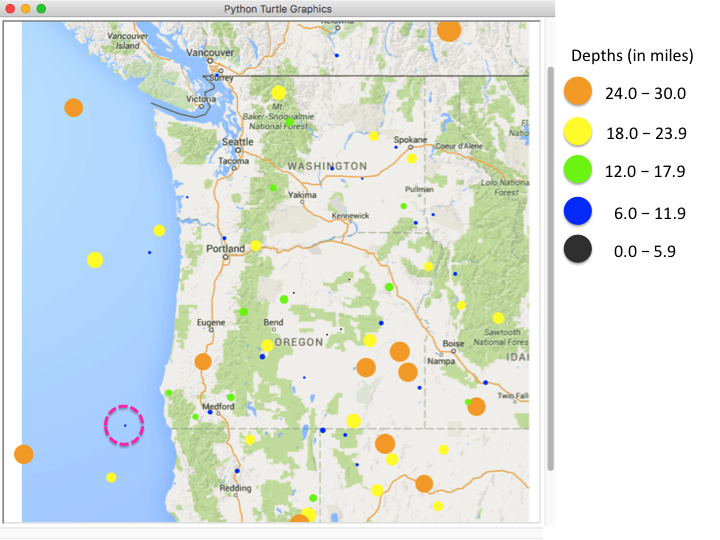
\includegraphics[scale=0.4]{depths-frequent-1.png}
\end{figure}
}

\frame{
\frametitle{\textbf{Magnitudes} \& Depths Frequent Occurrence}
\begin{figure}
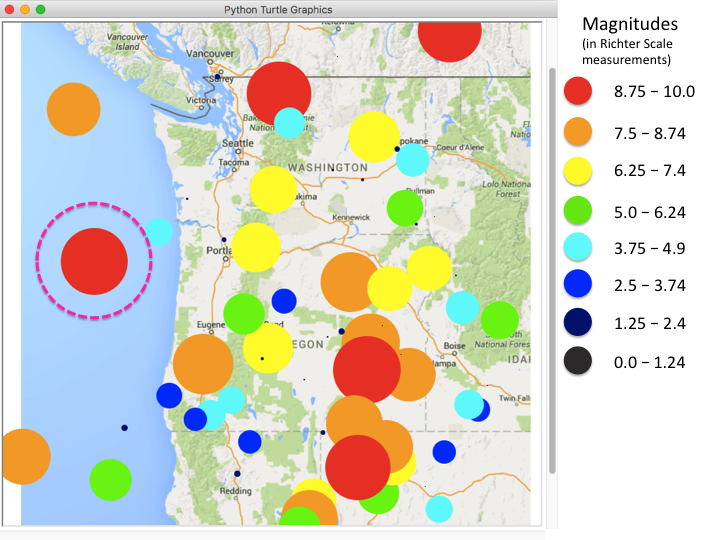
\includegraphics[scale=0.4]{mags-frequent-2.png}
\end{figure}
}

\frame{
\frametitle{Magnitudes \& \textbf{Depths} Frequent Occurence}
\begin{figure}
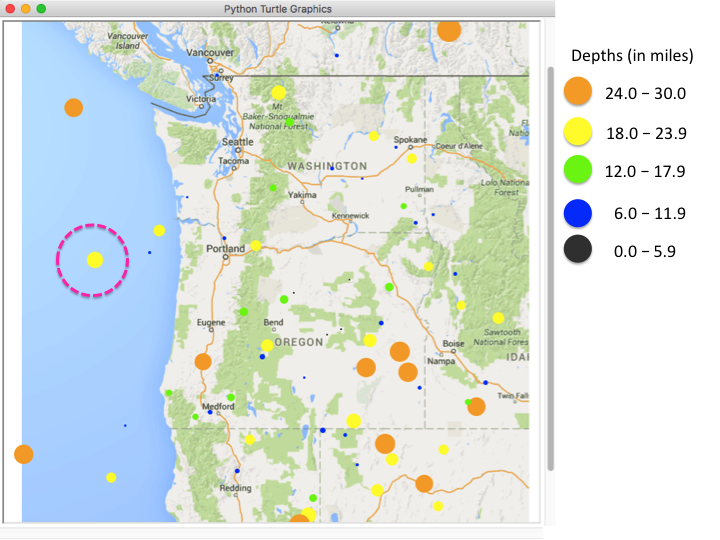
\includegraphics[scale=0.4]{depths-frequent-2.png}
\end{figure}
}

\frame{
\frametitle{\textbf{Magnitudes} \& Depths Outlier}
\begin{figure}
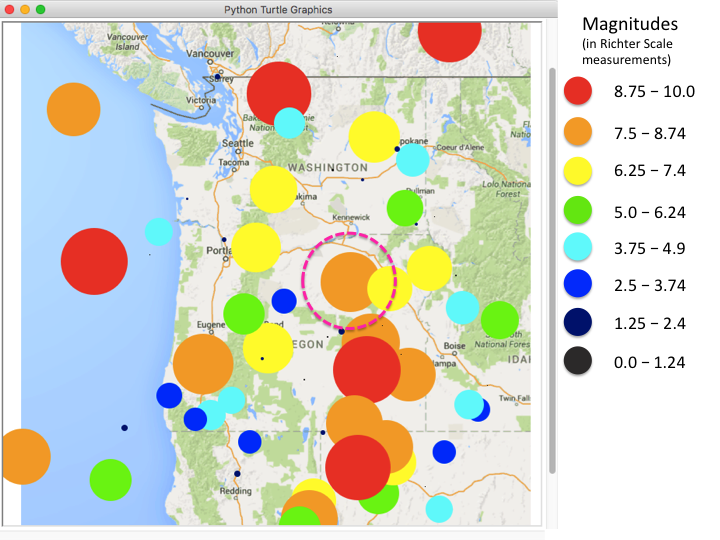
\includegraphics[scale=0.4]{mags-outlier.png}
\end{figure}
}

\frame{
\frametitle{Magnitudes \& \textbf{Depths} Outlier}
\begin{figure}
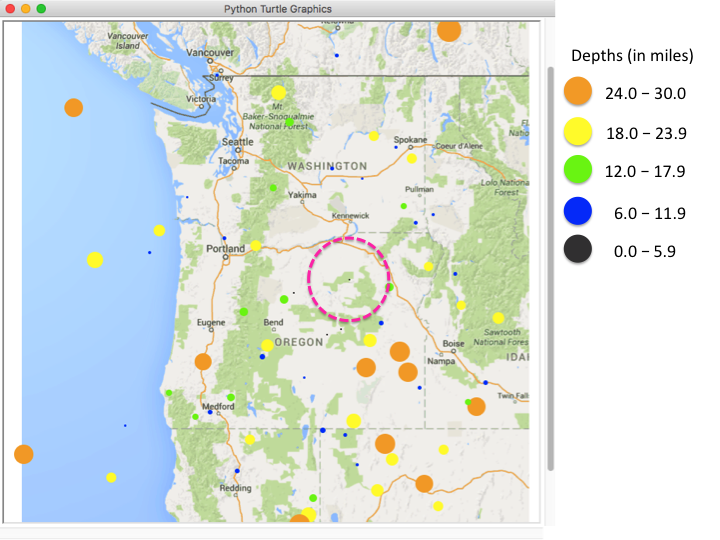
\includegraphics[scale=0.4]{depths-outlier.png}
\end{figure}
}


\frame{
\frametitle{Predict}
\begin{itemize}
\item North - Up
\item West - Left
\item East - Right
\item South - Down
\item right-slanted is high numbers
\item left-slanted is low numbers
\item right-leaning longitudes
\item left-leaning latitudes
\item Quakes drift towards lower-right corner
\end{itemize}
}

\frame{
\frametitle{Latitudes \& Longitudes}
\begin{figure}
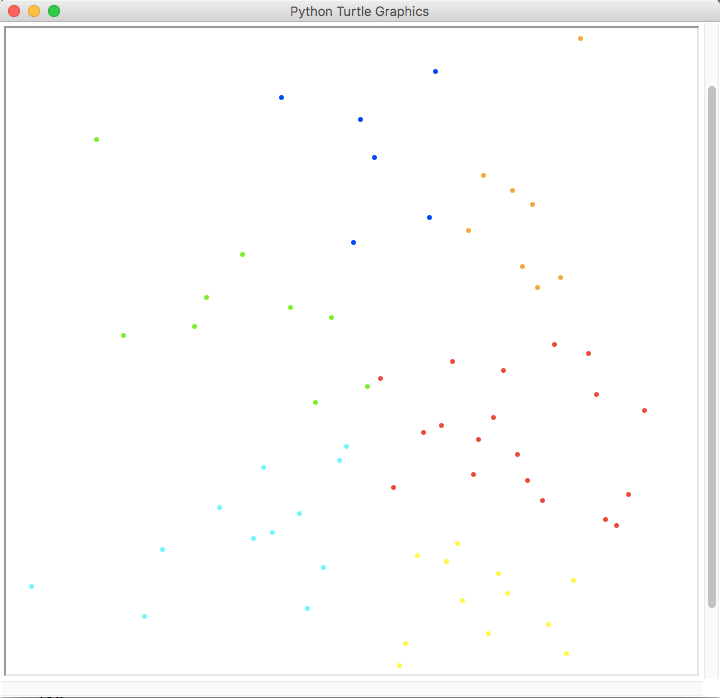
\includegraphics[scale=0.39]{clusters-nobg.png}
\end{figure}
}